\documentclass[notitlepage]{math}
\usepackage{lipsum}
\usetikzlibrary{patterns,positioning, decorations, decorations.pathreplacing}
\title{Function Local study Chap. 10} %Titre du fichie
\author{FireGhost} %Auteur du fichier

\begin{document}
\titre{Chapter 10: Function: Local study} %Titre du fichier .pdf
\UE{Function Local study} %Nom de la UE

\fairetitre
\fairemarges
% subsubsubsection
\setcounter{secnumdepth}{4}

\titleformat{\paragraph}
{\normalfont\normalsize\bfseries}{\theparagraph}{1em}{}
\titlespacing*{\paragraph}
{0pt}{3.25ex plus 1ex minus .2ex}{1.5ex plus .2ex}


\section{Continuity}
\subsection{First approach}
Let $f$ be a function from $I \subset R$ to $R$, we say that $f$ is continuous over $I$ if "the graph of $f$ can be drown without taking off the pencil from the paper".

\subsubsection{Example}
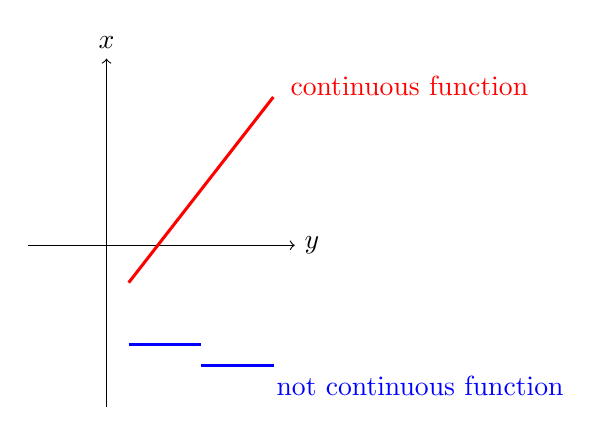
\begin{tikzpicture}[x=0.75pt,y=0.75pt,yscale=-1,xscale=1]
    %Straight Lines [id:da24929647938311184] 
    \draw  [->]  (189.3,210) -- (189.3,42.05) node[above] {$x$};
    %Straight Lines [id:da4428013785785254] 
    \draw  [->]  (151.6,132) -- (280,132) node[right] {$y$};
    %Straight Lines [id:da03148052252332034] 
    \draw[red,line width=1.1pt]  (200,150) -- (269.7,60.55) ;
    %Straight Lines [id:da8135470928175486] 
    \draw[blue,line width=1.1pt]    (200,180) -- (235,180) ;
    \draw[blue,line width=1.1pt]    (235,190) -- (270,190) ;
    %\draw[dashed]    (235,180) -- (235,190) ;
    
    % Text Node
    \draw[red] (276.7,49.2) node [anchor=north west][inner sep=0.75pt]    {continuous function};
    % Text Node
    \draw[blue] (270,193.7) node [anchor=north west][inner sep=0.75pt]    {not continuous function};
\end{tikzpicture} 
\subsection{Definition}
\begin{enumerate}[label=\protect\circled{\arabic*}]
    \item $f$ continuous at $a \in I$: \\ we say $f$ is continuous at $a$ - $a$ being a point of $I$ - if and only if:
    \begin{align*}
        f(a) &= \lim_{x \to a} f(x) \\
        f(a) &= \lim_{\begin{smallmatrix}
            x \to a \\
            x > a
        \end{smallmatrix}}f(x) = \lim_{\begin{smallmatrix}
            x \to a \\
            x < a
        \end{smallmatrix}}f(x) 
    \end{align*}
    \item $f$ continuous over $I$: \\ we say $f$ is continuous over $I \subset R$ if and only if $\forall a \in I$,$f$ is continuous at $a$.
\end{enumerate}
\subsection{Intermediate value theorem}
Let $f$ be a function continuous over $I \subset R$ and $(a,b) \in I^2$. if $f(a) f(b) < 0$ then there exists (at least one) $c$ from $]a,b[$ such that $f(c) = 0$.
\subsubsection{Examples}
\begin{minipage}{0.4\textwidth}  
    \begin{tikzpicture}[x=0.75pt,y=0.75pt,yscale=-1,xscale=1]
        %Straight Lines [id:da24929647938311184] 
        \draw  [->]  (189.3,160) -- (189.3,42.05) node[above] {$x$};
        %Straight Lines [id:da4428013785785254] 
        \draw  [->]  (151.6,132) -- (280,132) node[right] {$y$};
        %Straight Lines [id:da03148052252332034] 
        \node (a) at (200,150) {$a$};
        \node (b) at (270,60.55) {$b$};
        \draw[dashed,line width=1.1pt]  (205,155) -- (265,65) ;
        \node (text) at (195,190) {must intersect the x-axis};
    \end{tikzpicture}
\end{minipage}
\begin{minipage}{0.6\textwidth}
    Second example: $f(x) = x^2-2x+1$\\
    $f(x) = x^2 \cos(x)+x\sin(x)+1=0$ does f have any solutions?\\
    $I = [0,\pi]$ $f(a=0)=1$ and $f(b=\pi)=-\pi^2+1<0$
    \begin{enumerate}
        \item $f: x \mapsto f(x)$ is constant over $I \subset \mathbb{R}$.
        \item $f(a) \times f(b) < 0$. 
    \end{enumerate}    
    IVT $\Rightarrow \exists c \in ]0,\pi[, f(c) = 0$.
\end{minipage}
\section{Image of an interval by a continuous function}
Let $f : I \subset \mathbb{R} \to \mathbb{R}$ and $A \subset I$.\\
We call image of $A$ by $f$ and denote $f(A) : f(A) = \{f(x), x \in A\}$.
\subsection{Remark}
$\forall y \in f(A), \exists x \in A, y = f(x)$.
Example: $f: x \mapsto x^2$ and $A = [-3,2] \rightarrow f(A) = [0,9]$.
\subsection{Proposition}
\begin{itemize}
    \item The image of an interval by a continuous function is an interval.
    \item The image of a segment $([a,b])$ by a continuous function is a segment.
    counter example: $f: x \mapsto \frac{1}{x}$ (continuous over $\mathbb{R}^*_+$) \quad
    $f(]0,1] \subset \mathbb{R}^*_+) = [1,+\infty[$
\end{itemize}
\subsection{Corollary}
Let $f$ be a continuous function over segment $[a,b]$. Then $f([a,b]) = [m,M]$ where $m$ and $M$ are respectively the minimum and maximum of $f$ over $[a,b]$.
\section{Differentiability}
All function below are of type $f: I \to \mathbb{R}$ where $I$ is an interval of $\mathbb{R}$ containing at least two points.
\subsection{Definition}
we say that $f$ is differentiable at $a$ if the following quantity $\frac{f(x)-f(a)}{x-a}$ (the increasing rate of $f$ at $a$) has a finite limit $l$ at $a$.\\
If so, then $f$ is differentiable at $a$ and $f'(a) = l$ is called the derivative number of $f$ at $a$.
\subsubsection{Example}
\noindent $f : x \mapsto \sqrt{x}$ if $a = 0$ then: $\frac{f(x)-f(0)}{x-0} = \frac{\sqrt{x}-\sqrt{0}}{x-0} = \frac{\sqrt{x}}{x}= \frac{1}{\sqrt{x}} \rightarrow +\infty$ when $x \rightarrow 0$\\
$\forall a > 0, \frac{\sqrt{x}-\sqrt{a}}{x-a} = \frac{x-a}{(x-a)(\sqrt{x}+\sqrt{a})} = \frac{1}{\sqrt{x}+\sqrt{a}} \rightarrow \frac{1}{2\sqrt{a}}$ when $x \rightarrow a$\\
So $f : x \mapsto \sqrt{x}$ is differentiable at $a$ and $f'(a) = \frac{1}{2\sqrt{a}}$.
\subsubsection{Remarks}
\begin{enumerate}[label=\protect\circled{\arabic*}]
    \item If $f$ is differentiable at $a$, then the graph of $f$ has a non-vertical tangent at $a$.
    \item If the variation rate tends to $+\infty$ or $-\infty$, then the graph of $f$ admits a vertical tangent.
\end{enumerate}
\subsection{Differentiability and continuity}
\subsubsection{Proposition}
\begin{minipage}{0.35\linewidth}
    If $f$ is differentiable at $a$ then $f$ is continuous at $a$.
\end{minipage}
\hfill\vline\hfill
\begin{minipage}{0.54\linewidth}
    \begin{align*}
        \text{Differentiable} &\Longrightarrow \text{Continuity}\\
        &\;\not\!\!\!\Longleftarrow  
    \end{align*}
        ex: $\sqrt{x}$ at $0$ is continuous but not differentiable.
\end{minipage}
\subsubsection{Proof}
\begin{align*}
    \text{Differentiable} \implies \exists l \in \mathbb{R}, \lim_{x \to a} \left(\frac{f(x)-f(a)}{x-a}\right) = l &\implies \lim_{x \to a} \left(f(x) - f(a)\right) = 0\\
    &\implies \lim_{x \to a} \left(f(x)\right) = \lim_{x \to a} \left(f(a)\right)\\
    &\implies f \text{ is continuous at } a
\end{align*}
\section{Taylor Expansion}
\subsection{Taylor-Young Theorem}
Let $n \in \mathbb{N}$ and $f$ be a function of class $C^n$ over $I$ ($\textit{id est } f$ is differentiable at least $n$ times and $f^{(n)}$ is continuous over $I$).\\
Let $a \in I$ and $x \in I$. Then:
\[f(x) = f(a) + (x-a)f'(a) + \frac{(x-a)^2}{2!}f''(a) + \dots + \frac{(x-a)^n}{n!}f^{(n)}(a) + o((x-a)^n)\]
\subsubsection{Remark}
\begin{itemize}
    \item $n! = n \times (n-1) \times \dots \times 2 \times 1$, ex: $5! = 5 \times 4 \times 3 \times 2 \times 1 = 120$
    \item $f^{(n)} \leftarrow$ $n$-th derivative of $f$  ex: $f^{(3)} = f'''$.
    \item $o((x-a)^n) \leftarrow$ negligible quantity with respect to \[ {(x-a)}^n \implies \lim_{x \to a} \left(\frac{o((x-a)^n)}{(x-a)^n}\right) = 0\]
    \item Theorem mostly used with $a=0$.
\end{itemize}
\subsection{Definition of Taylor's expansion}
Let $n \in \mathbb{N}$, we say that $f$ admit a Taylor expansion of order $n$ at $a$ if there exists real numbers $a_0, a_1, \dots, a_n$ such that:
\[f(x) = a_0 + a_1(x-a) + a_2(x-a)^2 + \dots + a_n(x-a)^n + o((x-a)^n)\]
\subsubsection{Remarks}
We compute the coefficients $a_0, a_1, \dots, a_n$ using the Taylor-Young theorem for $f$.
\begin{align*}
    \text{for ex. } f: x \mapsto e^x &\implies a_0 = f(0) = e^0 = 1\\
    &\implies a_1 = f'(0) = e^0 = 1 \\
    &\implies a_2 = f''(2) = \frac{1}{2!}
\end{align*}
\[e^x = 1 + x + \frac{x^2}{2!} + \frac{x^3}{3!} + \dots + \frac{x^n}{n!} + o(x^n)\]
\begin{tikzpicture}
    \node (Let) at (-2, 0) {};
    \node (one) at (2, 1.5) {$e^x = 1 + x + $};
    \node[right = -0.1mm of one] (restOne) {$A(x)$};
    \draw [decorate, decoration={brace, mirror, raise=2.5pt}] (restOne.south west) -- (restOne.south east) node [midway,sloped,below = 0.15cm] {$o(x)$};
    
    \node (two) at (8, 1.5) {$e^x = 1 + x + x^2 + $};
    \node[right = -0.1mm of two] (restTwo) {$B(x)$};
    \draw [decorate, decoration={brace, mirror, raise=2.5pt}] (restTwo.south west) -- (restTwo.south east) node [midway,sloped,below = 0.15cm] {$o(x)$};
\end{tikzpicture}
\subsection{Usual function Taylor expansion at 0 <3}
\begin{itemize}
    \item ${\color{BurntOrange}e^x} = 1 + x + \frac{x^2}{2!} + \frac{x^3}{3!} + \dots + \frac{x^n}{n!} + o(x^n)$
    \item ${\color{BurntOrange}\cos(x)} = 1 - \frac{x^{\color{Red}2}}{2!} + \frac{x^{\color{Red}4}}{4!} + \dots + (-1)^n \frac{x^{2n}}{(2n)!} + o(x^{2n})$ {\color{Red} even function}
    \item ${\color{BurntOrange}\sin(x)} = x - \frac{x^{\color{Red}3}}{3!} + \frac{x^{\color{Red}5}}{5!} + \dots + (-1)^n \frac{x^{2n+1}}{(2n+1)!} + o(x^{2n+1})$ {\color{Red} odd function}
    \item ${\color{BurntOrange}\ln(1+x)} = x - \frac{x^2}{2} + \frac{x^3}{3} + \dots + (-1)^{n-1} \frac{x^n}{n} + o(x^n)$
    \item ${\color{BurntOrange}(1 + x )^{\alpha}} = 1 + \alpha x + \frac{\alpha(\alpha-1)}{2!} x^2 + \dots + \frac{\alpha(\alpha-1)\dots(\alpha-n+1)}{n!} x^n + o(x^n)$
    \item $\frac{1}{1-x} = 1 + x + x^2 + \dots + x^n + o(x^n)$
    \item $\frac{1}{1+x} = 1 - x + x^2 - \dots + (-1)^n x^n + o(x^n)$
\end{itemize}
\end{document}